\clearpage
\fancyhead[R]{\sffamily\small\color{Muted}Vulkan / 点光源与材质}
\section{带材质的逐灯与分簇绘制}

把三盏灯放在一块橙色金属板前，灯的半径依次取 6、4 和 3 个场景单位。这次先让每个像素按顺序检查三盏灯，再让分簇算法先查灯表。两边都从同一个点向灯检查遮挡，并读取同一份粗糙度、金属度。把板子换成粗糙金属或非金属后，双精度 CPU 程序仍可逐灯给出参照。CPU 采用 glTF 附录 B 的反射公式，独立计算表面能反进眼睛的亮度。

{\smalltable\noindent\begin{tabularx}{\linewidth}{@{}Xrrrr@{}}\toprule
橙色面板 & 中心红通道 & 分簇与逐灯最大差 & 单帧 MSE & 64 帧均值 MSE\\\midrule
非金属，粗糙度 0.25 & 1.170 & 0.0000725 & 0.01088 & 0.000396\\
金属，粗糙度 0.70 & 0.346 & 0.00000039 & 0.00416 & 0.000199\\
金属，粗糙度 0.25 & 16.105 & 0.000565 & 0.31989 & 0.004313\\\bottomrule
\end{tabularx}\par}

最大差取整幅 $33\times33$ 图像、三个线性 RGB 通道中的最大绝对值。后两列以 CPU 逐灯解为参考，比较一次 ReSTIR DI 输出，以及连续 64 帧的平均。中心高光最窄的那块面板，抽到正对镜头的灯与抽到侧灯会得到很不一样的亮度，因此单帧误差最大。这个场景检验了把材质高光计入选择权重后，增加样本能否让整张图接近参照。

RTX 5070 Ti Laptop GPU，Vulkan Debug x64。RenderDoc 1.47 的事件 8 逐灯绘制，22 建灯表，33 使用灯表绘制。对同一帧先预热一次、再回放 11 次，三步 GPU 时间中位数依次为 4.608、3.264、4.576 微秒。分簇的两步合计约 7.84 微秒，在三盏灯的小图上，建表已比它省下的着色工作耗时更长。增加灯数和画幅后需重测。

另起未挂 RenderDoc 的进程，两种方法交替先执行，预热四组后再各记 21 组。从发起计算到主线程等到结束，逐灯和分簇的中位数是 151.3 与 242.4 微秒。这段还包含命令提交、驱动与等待，不能作为纯 CPU 录制耗时。两光路有相同的阴影测试；实际放入一块完全遮住点光源的立方体时，板中心两处读数都为零。

\begin{figure}[H]\centering
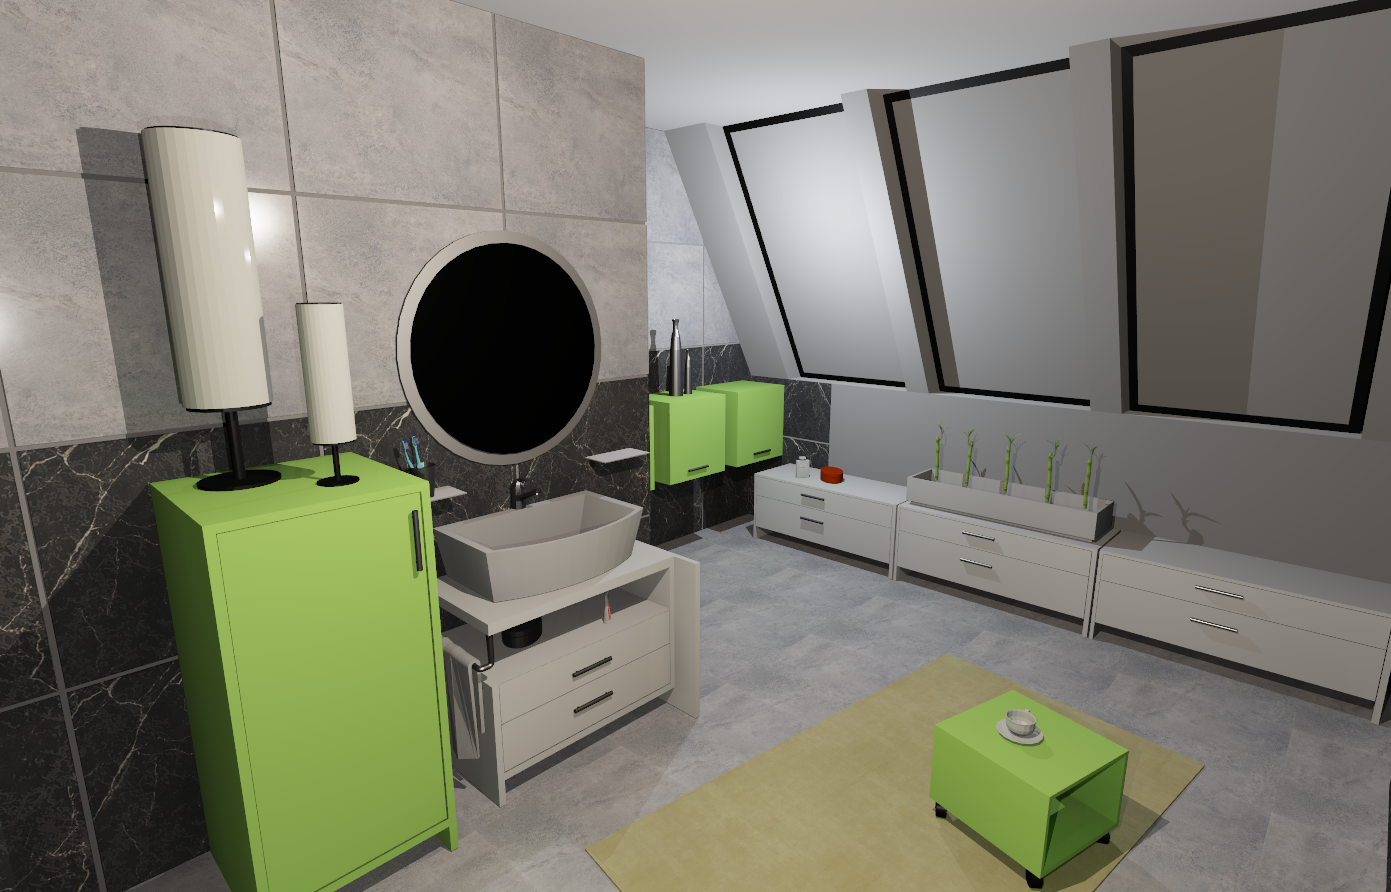
\includegraphics[width=.69\linewidth]{point-materials/bathroom-pbr.png}
\caption{把同一着色公式用到浴室的灯壳和柜门。实际编辑器重新打开已烘焙的场景，RenderDoc 第 12 帧，场景面板原图为 $1391\times892$。上表的计时取自三灯面板测试。}
\end{figure}

\readings{\href{run:../profiling/point-materials/renderdoc.json}{帧号、事件、全部 GPU 计时}\quad
\href{run:../profiling/point-materials/point-times.csv}{主线程计时}\quad
\href{run:../profiling/point-materials/point-materials.csv}{材质与误差}\quad
\href{run:../profiling/point-materials/README.md}{源码与复现方法}}
